\documentclass{beamer}

\usetheme{CambridgeUS}

\usepackage[utf8]{inputenc}
\usepackage[T1]{fontenc}

\usepackage{CJKutf8}
\usepackage{datetime}
\usepackage{amsmath}
\usepackage{amssymb}
\usepackage{mathtools}
\usepackage{subcaption}
\usepackage{minted}
\usepackage{xcolor}
\usepackage{ulem}
\usepackage{hyperref}
\usepackage{graphicx}
\usepackage{cite}
\usepackage{multirow}
\usepackage{makecell}
\usepackage{url}
\usepackage{placeins}

\graphicspath{{images/}}
\DeclareGraphicsExtensions{.pdf}

\newdate{date}{03}{06}{2025}
\date{\displaydate{date}}
\title[Fairness]{Quantitative Auditing of AI Fairness with Differentially Private Synthetic Data}
\author[Rex]{
    \begin{CJK}{UTF8}{bsmi}袁至誠\end{CJK}\newline
    Chih-cheng Rex Yuan\newline
    \href{https://rexyuan.com/}{rexyuan.com}
    }
\institute[IIS,AS]{Institute of Information Science, Academia Sinica}

\DeclarePairedDelimiter{\set}{\{}{\}}
\DeclarePairedDelimiter{\tuple}{(}{)}
\DeclarePairedDelimiter{\abs}{\lvert}{\rvert}

\let\oldleq\leq
\renewcommand{\leq}[1][]{\oldleq_{#1}}
\renewcommand{\implies}{\rightarrow}

\newcommand{\bye}[1]{}

\newcommand{\red}[1]{\textcolor{red}{#1}}
\newcommand{\sred}[1]{\textcolor{red}{\sout{#1}}}

\begin{document}

\begin{frame}
\titlepage
\end{frame}

\begin{frame}{Why Fairness Audits Matter}
  \begin{itemize}
    \item AI systems are influencing justice, health, finance.
    \item Bias in AI means real-world discrimination.
    \item Example: COMPAS audit by ProPublica.
  \end{itemize}
\end{frame}

\begin{frame}{Auditing Framework Overview}
    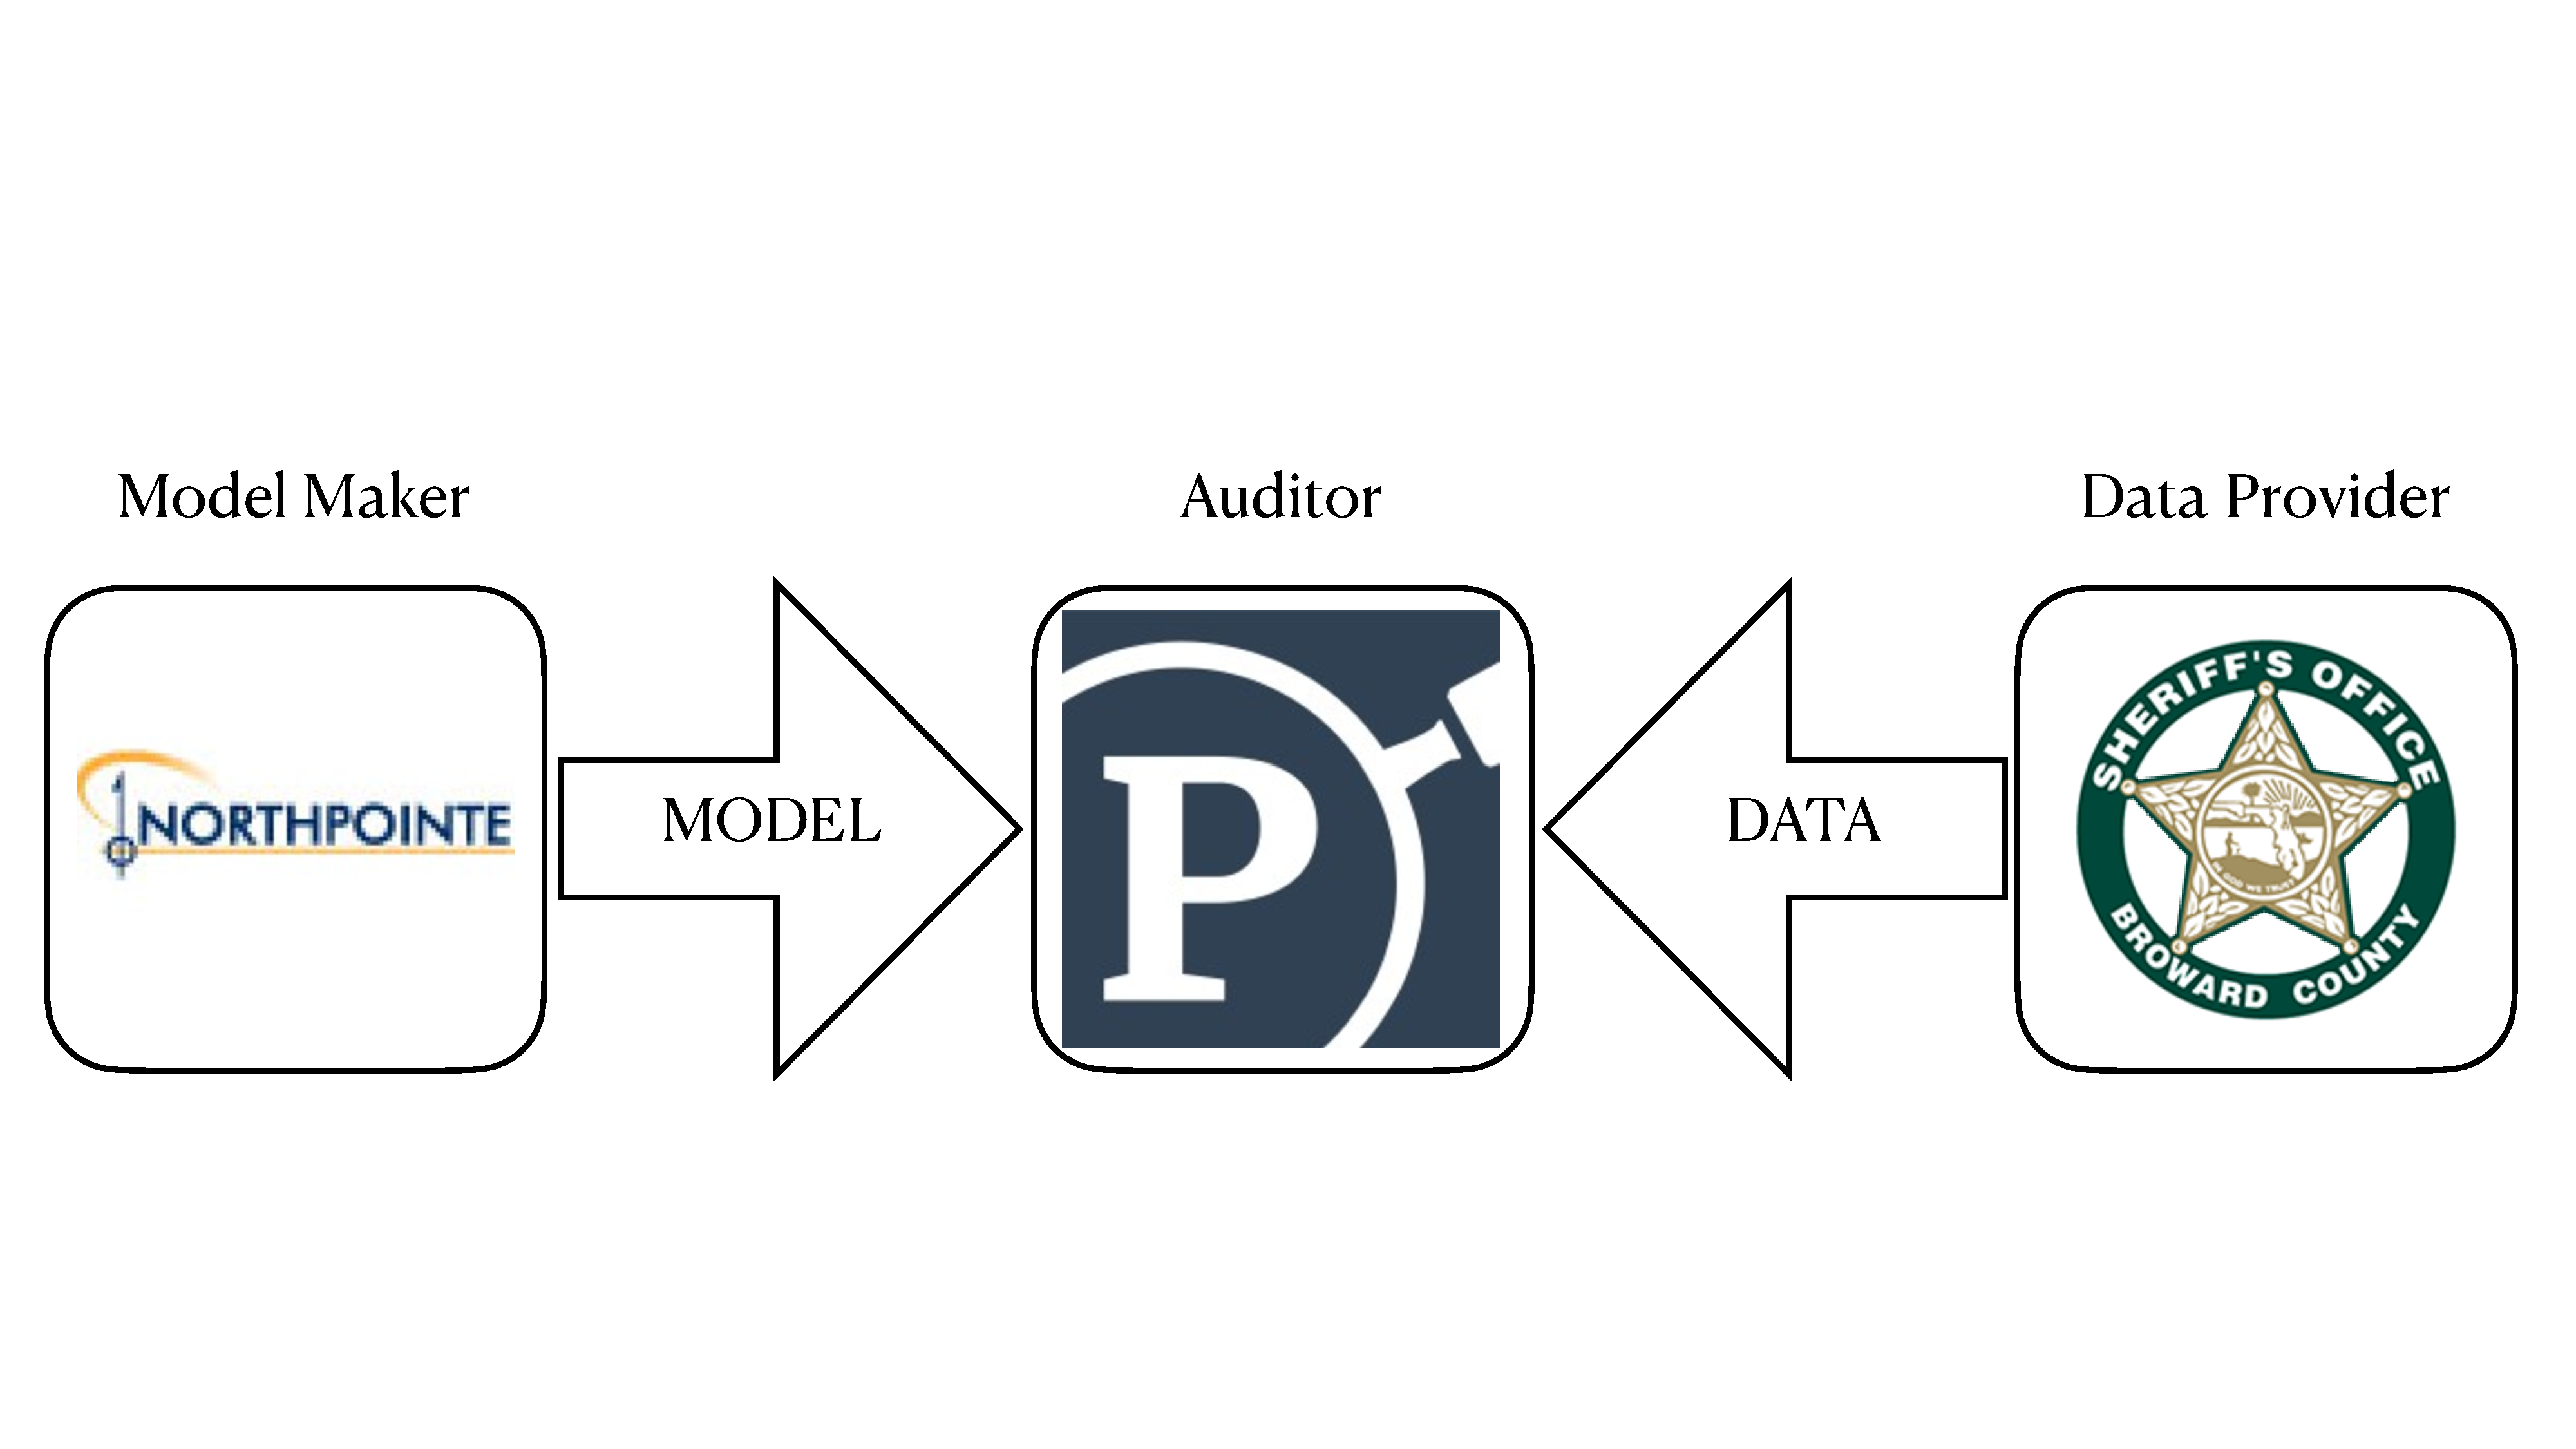
\includegraphics[width=\linewidth]{compas}
\end{frame}

\begin{frame}{The Privacy Problem}
  \begin{itemize}
    \item Auditors need sensitive data to test fairness.
    \item But holding this data introduces security and privacy risks.
    \item Security risk: hackers could steal the data.
    \item Privacy risk: published stats could expose insights.
  \end{itemize}
\end{frame}

\begin{frame}{Solution: Privacy-Preserving Audits}
  \begin{itemize}
    \item Use synthetic data generated from real data.
    \item Apply differentially private synthetic data to ensure individual info stays hidden.
    \item Auditors only keep the synthetic data and not the real data.
  \end{itemize}
\end{frame}

\begin{frame}{What Is Differentially Private Synthetic Data?}
  \begin{itemize}
    \item Fake data that mimic the real data's patterns.
    \item Generated with differential privacy, which adds noise to protect privacy.
    \item Lets auditors analyze fairness without exposing personal data.
  \end{itemize}
\end{frame}

\begin{frame}{How The Synthetic Data Are Generated}
  \begin{itemize}
    \item We use a proven method that won a U.S. government competition (NIST, 2018).
    \item It adds noise to protect privacy while preserving overall patterns.
    \item The result: data that looks real but contains no real individuals.
  \end{itemize}
\end{frame}

\begin{frame}{Does It Work?}
  \begin{itemize}
    \item Compared fairness metrics on real and synthetic data.
    \item Datasets: Adult, COMPAS, Diabetes.
    \item Most metrics are within negligible difference.
  \end{itemize}
\end{frame}

\begin{frame}{Policy Implications}
  \begin{itemize}
    \item Enables safer third-party audits under privacy guarantees.
    \item Avoids liability for storing sensitive datasets.
  \end{itemize}
\end{frame}

\begin{frame}{Conclusion}
  \begin{itemize}
    \item Synthetic data can support fairness audits with privacy.
    \item Our framework is practical and provably private.
    \item Opens new pathways for legal oversight of AI systems.
  \end{itemize}

  Slides: \url{https://github.com/RexYuan/Eunectes}.
\end{frame}

\end{document}
